%\section{Introduction}

Laser frequency stabilisation is an essential tool for atomic physics experiments, without it experiments involving \glspl{bec}, atomic clocks and many more would not be possible~\cite{anderson_observation_1995,ye_quantum_2008}.
There are a plethora of techniques available for laser frequency stabilisation each with numerous advantages and disadvantages.

Laser frequency stabilisation is an essential component of the \gls{caeis} as it is required for the \gls{mot} to function, for imaging of the atomic cloud and for the precise control involved in the ionisation process.
Relatively simple techniques such as saturated absorption spectroscopy are adequate for the frequency linewidths required for the \gls{mot}.
More precise methods are useful when interacting with the Rydberg states of an atom as the difference in energy between states becomes small for high-lying states and thus a narrow linewidth laser is required to precisely interact with a single state.

\Gls{pdh} locking with a high-finesse cavity is a proposed method for precise control over a laser's frequency with a \gls{caeis}.
\Gls{pdh} has been used to produce extremely good frequency stabilisation with sub-\unit[40]{mHz} linewidths achieveable~\cite{kessler_sub-40-mhz-linewidth_2012}.
The \gls{pdh} technique is unfortunately not relative to an absolute frequency reference, such as a atomic frequency, which allows the frequency of the laser to drift with ambient changes.
In order to capitalise on the narrow linewidth achieveable with \gls{pdh} locking an absolute frequency reference, such as saturated absorption spectroscopy or polarisation spectroscopy is required in combination with \gls{pdh} to prevent slower drifts due to changes in the optical cavities resonance as temperature and pressure changes in the lab.

The focus of this chapter is on \gls{ps} which was first described by Wieman and H\"anch in 1976 as, ``...a sensitive new method of Doppler-free spectroscopy, monitoring the nonlinear interaction of two monochromatic laser beams in an absorbing gas via changes in light polarisation."~\cite{wieman_doppler-free_1976,demtroder_laser_2003}.
This chapter provides an overview of laser frequency stabilisation, a detailed discussion of the physics of \gls{ps} followed by details on the implementation and measurement of high bandwidth frequency stabilisation using \gls{ps}.
Much of the work described in this chapter was conducted in collaboration with MogLabs using MogLabs' diode lasers and control electronics.
This research was instrumental in improving the bandwidth of the electronics headboard used in MogLabs lasers which was required to achieve an order of magnitude improvement in the linewidth previously achieved with \gls{ps}~\cite{torrance_sub-kilohertz_2016}.

\section{Laser Frequency Stabilisation}

Laser frequency stabilisation describes a number of techniques that are used to reduce the frequency spread of a laser's frequency.
This can range from weak frequency stabilisation keeping the centre frequency of a laser at a particular frequency to convoluted frequency narrowing techniques that attempt to reduce laser linewidth to sub-hertz levels.
Typically these techniques use some reference to measure frequency deviation from a given frequency and provide negative feedback to the laser, using a servo system, to keep it at the target frequency.

The efficacy of stabilisation techniques can be described by the width of the frequency distribution of the laser, called the linewidth.
Linewidth usually refers to either the \gls{fwhm} or \gls{rms} width about the central frequency and is used to descibe measurements made over various timescales.
Short measurements, usually less than a second measurement, are used to describe the linewidth of laser whereas long timescale measurement, hours or days in duration, are used to describe the drift of the laser central frequency over time.

There are a number of traits that are desirable in a laser frequency stabilization scheme including the ability to stabilize to an absolute atomic reference, absence of frequency or amplitude modulation, high bandwidth to achieve low spectral linewidth, large capture range, low complexity and low cost.

There are a large number of available techniques and variations on techniques for stabilization each with different advantages and drawbacks.
A few of these techniques are \gls{sa}~\cite{haroche_theory_1972, maguire_theoretical_2006, cuneo_optically_1994, preston_doppler-free_1996, saliba_linewidths_2009}, \gls{davll}~\cite{corwin_frequency-stabilized_1998, millett-sikking_davll_2007}, \gls{mts}~\cite{shirley_modulation_1982, mccarron_modulation_2008, xiang-hui_ultra-stable_2009,negnevitsky_wideband_2013}, Sagnac interferometry~\cite{robins_Interferometric_2002, jundt_non-linear_2003}, \acrfull{ps}~\cite{wieman_doppler-free_1976, lancaster_polarisation_1999, yoshikawa_frequency_2003, harris_polarization_2006, pearman_polarization_2002, tiwari_laser_2006, do_polarization_2008, torii_laser-phase_2012}, \gls{pdh}~\cite{drever_laser_1983}, and H\"ansch Couillaud stabilisation~\cite{hansch_laser_1980}.

\subsection{Frequency Control and Feedback}

There are a number of methods to control the output frequency of a laser and these can be used to supply feedback from the stabilisation technique in order to decrease the linewidth of a laser system.
The focus here will be on the feedback systems of diode lasers, particularly \glspl{ecdl}.

\subsubsection{Temperature}
The temperature of a laser diode affects the output frequency due to the temperature dependence of the optical path length and gain curves~\cite{wieman_using_1991}.
The two processes affect output frequency at different rates and both show an increase in wavelength with increasing temperature.

The temperature of laser diodes can be controlled through two methods. \Glspl{tec} can be used to directly control the temperature of the device and the injection current into the diode affects the temperature. Good insulation and thermal inertia also contribute to the stability of diode temperature~\cite{saliba_cold_2011}.

Temperature is not typically used to directly manipulate the frequency of a laser due to the relatively slow response as changes in the control signal take seconds to propagate from the \gls{tec} to the diode and longer to fully thermalise.
Typically temperature is just stabilised to reduce the impact of ambient temperature changes on the performance of the diode laser.

\subsubsection{Injection Current}
Modulation of the injection current into the laser diode is one of most common ways of controlling the output wavelength of a diode laser.
The injection current into the diode affects the temperature of the diode and the density of charge carriers which in turn affects the refractive index of the medium and thus the wavelength of the laser light produced.

Modulation of the injection current is the fastest feedback method available to diode lasers and is able to suppress noise up to \unit{MHz} ranges~\cite{ludlow_compact_2007,torrance_sub-kilohertz_2016}.
The design of the electronics involved in the modulation of the injection current can have a noticeable influence on the performance at high frequencies as noise becomes an issue.
{\color{red}See section something that discusses improvements made to the design of the electronics used in the MogLabs lasers used in this research.}

\subsubsection{Grating Angle}
In external cavity diode lasers, for example Littrow configuration \glspl{ecdl} as shown in Figure~\ref{figure:littrow}, the angle of the external grating can be used to control the output frequency.
The grating angle affects the wavelength of the light that is reflected back into the laser diode and thus the angle can be used to select output wavelength.
The grating angle is commonly controlled using piezoelectric actuators~\cite{hawthorn_littrow_2001}.

\begin{figure}
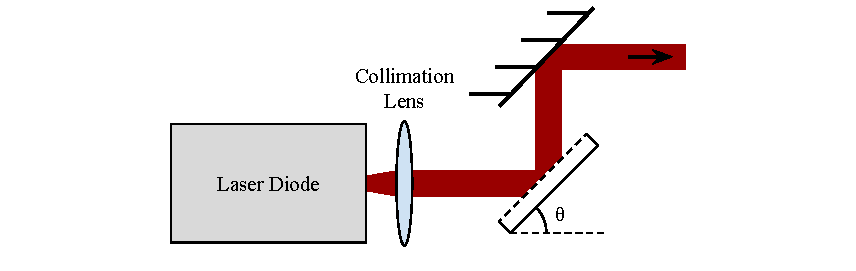
\includegraphics{part1/Figs/LittrowConfiguration.pdf}
\caption{Littrow configuration for diode lasers. The raw output of the diode is collimated and then incident on an optical grating. The angle of the grating, $\theta$, changes what frequency of light is coupled back into the diode and thus the frequency of output.
{\color{red}I'm not convinced this is entirely correct. Cavity length changed instead?}}
\label{figure:littrow}
\end{figure}

Frequency control by controlling the grating angle is limited by the response rate of the piezo actuator which tend to respond in microseconds.
Thus the grating angle can be used to deal with relatively low frequency noise, up to approximately \unit[100]{kHz} or so, such as changes to ambient temperature or pressure.

\subsection{Noise}
In this context noise refers to effects that change the frequency of a laser in undesireable ways.
Some sources of noise are thermal changes, ambient vibrations, atmospheric pressure, or changes in the electrical power supply.

Thermal noise can be causes by changes in weather, unreliable building climate control, or unexpected behaviours in thermal management devices (a malfunctioning \gls{tec} for example).
Thermal noise can affect the alignment of optics, the efficiency and polarisation of light transmitted through fibres, atomic vapour cell opacity and the intensity and frequency of light emitted from laser diodes all of which can affect the frequency of a stabilised laser system.

Electrical noise can occur with changes to the wider electrical grid as well as when devices in the lab are turned on or off, fast switching high-voltage/-current supplies, such as those used to switch the \gls{mot} coils, can cause noticeable affects on other electrical equipment in close proximity.
Noise in the electronic environment can cause frequency instability particularly if a laser diode is not fully isolated from the electrical ground. Noise on the power supply to the laser diode affects the intensity and frequency of the light emitted.
Laser intensity noise can also cause problems, for example laser frequency stabilisation is often conducted with spectroscopic techniques that will interpret intensity fluctuations as frequency fluctuations. Thus the feedback system will create frequency noise as it attempts to correct for the phantom frequency nosie.

Mechanical noise can have numerous sources such as audible noise, percussive noise (dropped spanners, doors) or vibrational sources such as cooling fans on nearby equipment.
\Glspl{ecdl} subjected to mechanical vibrations will experience frequency noise as the alignment of the light coupled back into the diode from the grating varies.
Mechanical noise can also affect the alignment, and thus transmitted power, of laser through optical fibres, optical isolators and apertures.

\section{Saturated Absorption Spectroscopy}
\glsreset{sa}
\Gls{sa} is a simple and common technique for laser frequency stabilisation which can be used with a number of atomic species and is a staple of atom optics laboratories~\cite{demtroder_laser_2003}.
\Gls{sa} is often used in applications where extremely narrow linewidths are not required due to the relative simplicity of the method such as \gls{mot} trapping and cooling, or atom cloud imaging.
A schematic of \gls{sa} is shown in Figure~\ref{figure:satabs}.

\begin{figure}
\center
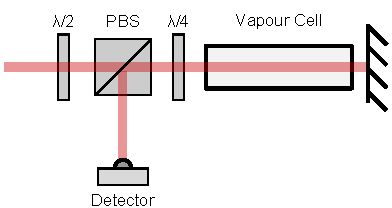
\includegraphics{part1/Figs/SatAbs.pdf}
\caption{An example of a saturated absorption spectroscopy setup. $\lambdaup$/2 and $\lambdaup$/4 refer to half- and quarter wave phase retarders respectively and are used to control the intensity of the light travelling through the vapour cell and hitting the detector using the polarising beam splitter (PBS).}
\label{figure:satabs}
\end{figure}

\Gls{sa} involves counter-propagating pump and probe beams from the laser source through a sample of atomic vapour with the intensity of the probe beam after the gas measured by a photodetector.
Without the pump beam the absorption of the probe as a function of laser frequency would show peaks at the atomic transitions, with width equal to the linewidth of each transition, smeared out by the thermal distribution of the atoms due to thermal motion which for room temperature atoms results in a smooth curve 100s of MHz wide which obscures the hyperfine transitions.
Adding the pump beam results in less absorption at each transition due to the pump exciting atoms which are then inaccessible to the probe. With counter-propagating beams `cross-over' features appear halfway between each pair of transitions.
An example spectrum for rubidium-85 is shown in Figure~\ref{figure:satabsspectrum}.
In Figure~\ref{figure:satabs} the pump beam is recycled to act as the probe.

\begin{figure}
    \center
    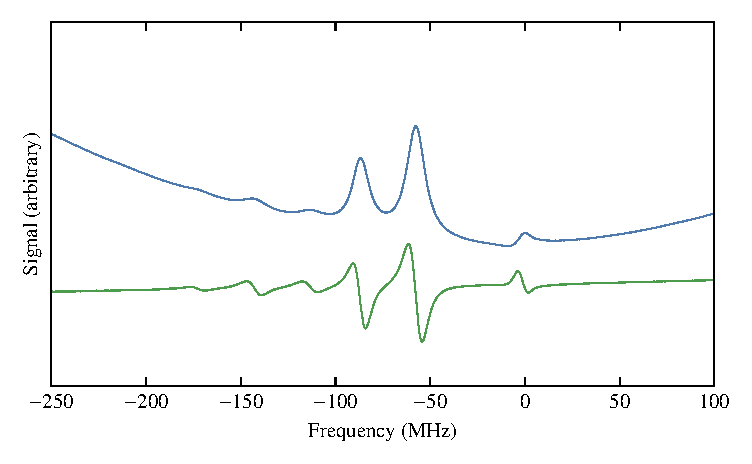
\includegraphics{part1/Figs/SatAbsSpectrum.pdf}
    \caption{An example of a saturated absorption spectroscopy absorption spectrum for the rubidium-85 D2 transition.
    The blue line shows the absorption spectrum and the green line shows the error signal for modulated \gls{sa}.
    From left to right the peaks in the absorption spectrum are the $F=3$ to $F'=2,2/3,3,2/3,3/4$, and $4$, where $x/y$ refers to a crossover transition.}
    \label{figure:satabsspectrum}
    % Code and data in Code/PolSpec Code/Laser/Spectra for Paper/Grapher.py
\end{figure}

Different variations of \gls{sa} can operate with or without modulation, which can be modulation of the laser itself or modulation of the transition frequencies of the atoms in the vapour cell (via a solenoid magnet wrapped around the vapour cell).
Without modulation the system is more susceptible to drift and there is an frequency offset from centre of the atomic transition.
If modulation is used then there is the added complexity of implementing the modulation and the potential linewidth is limited by modulation frequency.
Linewidths under \unit[150]{kHz} are easily attainable with modulated saturated absorption spectroscopy~\cite{saliba_linewidths_2009}.

\section{Pound Drever Hall}

The \gls{pdh} technique is the gold-standard for laser frequency linewidth reduction~\cite{drever_laser_1983} and has been used to achieve extremely low linewidth of less than \unit[40]{mHz}~\cite{kessler_sub-40-mhz-linewidth_2012}.
\Gls{pdh} uses an optical cavity as a frequency reference and a modulated beam and some electronics to generate the error signal for feedback to the laser.

\subsection{Fabry-P\'erot Cavities}{
A Fabry-P\'erot cavity is formed by two highly reflective mirrors facing each other such that light can form a standing wave between the two mirrors.
Laser light incident on a Fabry-P\'erot cavity will only couple into the cavity if the length of the cavity is equal to an integer number of wavelengths of the light.
So for an ideal laser to be resonant with an ideal cavity,
\begin{equation}
L = n \lambda,
\end{equation}
where $L$ is the length of the cavity, $\lambda$ is the wavelength of the laser and $n$ is some integer.
Realistic lasers and cavities have finite linewidths which when viewed as a transmission or reflection spectrum are shown as a convolution of the cavity and laser linewidth.

The frequency difference between one cavity tranmission and the next is called the \gls{fsr}, $\Delta \nu_{FSR}$ and depends on the length of the cavity,
\begin{equation}
\Delta \nu_{FSR} = \frac{c}{2L}
\end{equation}
The quality of an optical cavity is described by the cavity Finesse, $\mathscr{F}$, which effectively describes the number of traversals a beam makes before leaking out or being absorped and it is determined by the reflectivity of the mirrors, $R$,
\begin{align}
\mathscr{F} &= \frac{2\pi}{-\log_e\left(R^2\right)} \notag\\
 &= \frac{\Delta \nu_{FSR}}{\delta},
\end{align}
where $\delta$ is the \gls{fwhm} linewidth of the cavity.

The light transmitted through an optical cavity can be described by~\cite{pedrotti_introduction_2007}
\begin{equation}\label{equation:cavity_transmission}
T = \frac{1}{1+F\sin^2\frac{d}{2}},
\end{equation}
where $d=2\pi\frac{2L}{\lambda}$ and $F=\frac{4R}{\left(1-R\right)^2}$ is the coefficient of finesse.
The coefficient of finesse is related to the finesse by
\begin{equation}
\mathscr{F}=\frac{\pi}{2}\sqrt{F}.
\end{equation}
The phase difference between successive traversals of the cavity is represented by $d$
We can define the difference between the laser wavelength and closest cavity resonance as $\Delta\lambda=L-n\lambda$, then Equation~\ref{equation:cavity_transmission} can be written as
\begin{equation}
T = \frac{1}{1+F\sin^2\left(2\pi\frac{\Delta\lambda}{\lambda}\right)}.
\end{equation}
$T$ takes the form of a Lorentzian, or Airy, function and an example spectra is shown in Figure~{\color{red}[make cavity transmission figure]}

The cavity used in the experiments described in this chapter was a high-finesse cavity from Stable Laser Ssystems that was located inside an evacuuated temperature-controlled can.
This cavity has a finesse of 20942, a \gls{fsr} of \unit[1.5]{GHz}, a \gls{fwhm} linwidth of \unit[71.6]{kHz}, and the mirrors had a reflectivity of 0.99985.
}

\subsubsection{PDH Error Signal}

The magnitude of the electric field incident on a Fabry-P\'erot cavity, if the frequency is assumed to be approximately constant, can be written as
\begin{equation}
E_{I} = E_0 e^{i\omega t},
\end{equation}
where $\omega=2\pi f_l$ is the angular frequency of the laser.
The light reflected from the cavity consists of the promptly reflected beam and the leakage beam from light that has traversed the cavity one or more times before leaking out of the first mirror.
The promptly reflected beam undergoes a phase shift of $\pi$ relative to the incident beam.
The leakage beam has numerous phase components with one cavity round trip giving a phase shift of $-2L\omega/c$, two round trips giving $-4L\omega/c$, and so on.
Thus the reflected beam electric field will be
\begin{equation}\label{equation:cavity_reflected_field}
E_R = E_0 \left( r e^{i\left(\omega t + \pi\right)} + t r t e^{i\left(\omega t -2L\omega/c\right)} + t r^3 t e^{i\left(\omega t -4L\omega/c\right)} + ...\right),
\end{equation}
where $r$ is the mirror reflectivity and $t=\sqrt{1-r^2}$ is the transmissivity of the mirrors.
Equation~\ref{equation:cavity_reflected_field} can be simlified to give the reflection coefficient
\begin{equation}
F(\omega) \equiv \frac{E_R}{E_I} = \frac{r\left(e^{i\omega / \Delta\nu_{FSR}} - 1 \right)}{1-r^2 e^{i\omega / \Delta\nu_{FSR}}}.
\end{equation}
Figure {\color{red}[reference figure]} shows that $F(\omega)$ is antisymettric about the cavity resonance making it ideal for frequency stabilisation however more steps are required to generate a useable error signal.

To generate the error signal phase modulation is imposed on the laser, typically using an \gls{eom}.
The modulated incident laser beam with a modulation frequency of $\Omega/2\pi$ and modulation strength $\beta$ has electric field
\begin{align}
E_I &= E_0 e^{i\left(\omega t + \beta \sin\Omega t \right)} \notag \\
&\approx E_0 \Bigg( J_0(\beta) + 2iJ_1(\beta)\sin\Omega t \Bigg)e^{i\omega t} \notag \\
&= E_0 \Bigg( J_0(\beta)e^{i\omega t} + J_1(\beta)e^{i(\omega + \Omega)t} - J_1(\beta)e^{i(\omega - \Omega)t} \Bigg),\label{equation:cavity_phase_mod}
\end{align}
valid for small $\beta$ where $J_0$ and $J_1$ are Bessel functions.
Equation~\ref{equation:cavity_phase_mod} shows that the phase modulated beam has three frequency components and the two $J_1$ components are reffered to as the `sidebands' which are offset from the central frequency by the modulation frequency $\Omega/2\pi$.

The reflected beam from the cavity due to the phase-modulated beam results in each frequency component being transformed by $F(\omega)$ to give
\begin{equation}
E_R = E_0 \Bigg(F(\omega)J_0(\beta)e^{i\omega t} + F(\omega+\Omega)J_1(\beta)e^{i(\omega+\Omega) t} - F(\omega-\Omega)J_1(\beta)e^{i(\omega-\Omega) t} \Bigg).
\end{equation}
The electric field is not directly measured however, photodetectors measure the power, $P=|E|^2$ of the beam incident on them.
Thus,
\begin{align}
P_R = \,&P_c|F(\omega)|^2 \quad+\quad P_s \Bigg( F(\omega+\Omega) + F(\omega-\Omega)\bigg) &+\quad&\notag\\
& 2\sqrt{P_cP_s} \, \operatorname{Re}\Bigg[ F(\omega)F^*(\omega+\Omega)-F^*(\omega)F(\omega-\Omega)\Bigg]\cdot\cos\Omega t &+\quad& \notag\\
& 2\sqrt{P_cP_s} \, \operatorname{Im}\Bigg[ F(\omega)F^*(\omega+\Omega)-F^*(\omega)F(\omega-\Omega)\Bigg]\cdot\sin\Omega t &+ \quad&O[2\Omega]
\end{align}


\begin{figure}
\centering
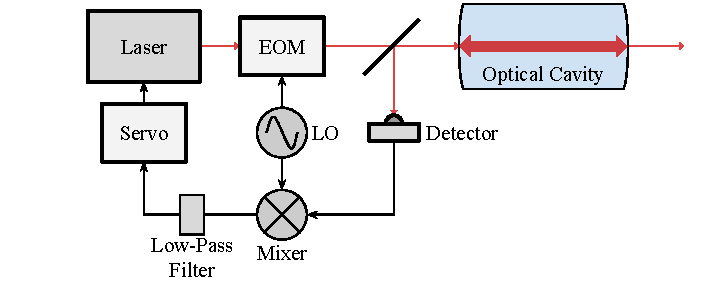
\includegraphics{part1/Figs/PDH.pdf}
\caption{A beautiful \gls{pdh} schematic.}
\end{figure}



